\documentclass[journel,12pt,twocoloums]{IEEEtran}

\title{Assignment 7-Probability and Random Variable}
\author{Annu-EE21RESCH01010}
\date{13 January 2020}

\usepackage{amsthm}
\usepackage{graphicx}
\usepackage{mathrsfs}
\usepackage{txfonts}
\usepackage{stfloats}
\usepackage{pgfplots}
\usepackage{cite}
\usepackage{cases}
\usepackage{mathtools}
\usepackage{caption}
\usepackage{enumerate}	
\usepackage{enumitem}
\usepackage{amsmath}
\usepackage[utf8]{inputenc}
\usepackage[english]{babel}
\usepackage{multicol}
%\usepackage{xtab}
\usepackage{longtable}
\usepackage{multirow}
%\usepackage{algorithm}
%\usepackage{algpseudocode}
\usepackage{array,multirow}
\usepackage{enumitem}
\usepackage{mathtools}
\usepackage{gensymb}
\usepackage{hyperref}
%\usepackage[framemethod=tikz]{mdframed}
\usepackage{listings}
    %\usepackage[latin1]{inputenc}                                 %%
    \usepackage{color}                                            %%
    \usepackage{array}                                            %%
    \usepackage{longtable}                                        %%
    \usepackage{calc}                                             %%
    \usepackage{multirow}                                         %%
    \usepackage{hhline}                                           %%
    \usepackage{ifthen}                                         %%
  \providecommand{\nCr}[2]{\,^{#1}C_{#2}}
  \providecommand{\nPr}[2]{\,^{#1}P_{#2}}
  \lstset{
%language=C,
frame=single, 
breaklines=true,
columns=fullflexible
}

 \begin{document}
 \maketitle
\textbf{Download latex code from here-}\\
\begin{lstlisting}
 https://github.com/annu100/AI5002-Probability-and-Random-variables/tree/main/ASSIGNMENT_7
 \end{lstlisting}
 \textbf{download python code from here}\\
 \begin{lstlisting}
  https://github.com/annu100/AI5002-Probability-and-Random-variables/blob/main/ASSIGNMENT_5/assignment_7.py
 \end{lstlisting}
 \section{Problem Statement-Problem 6.10}
 Let E and F be events with P(E) =$\frac{3}{5}$
, P(F) =$\frac{3}{10}$
and P(E \cap F) =$\frac{1}{5}$
. Are E and F independent?
Simulation part -
Also generate random variables according to normal distribution and check sum of 2 random variables is also normal.
\section{SOLUTIONS}
\subsection{Probability calculation}
We know that for independent random variables,multiplication of probability 2 random variables must be equal to multiplication of individual probability of those random variables.
P(E) =$\frac{3}{5}$
P(F) =$\frac{3}{10}$
P(E \cap F) =$\frac{1}{5}$
\begin{align}
       let    X &= P(E)*P(F) \\
                &=\frac{3}{5}*\frac{3}{10}
\end{align}
\\
But from above results,X is not equal to P(E \cap F).
\\


Therefore, $E$ and $F$ are not independent random variables.
It can be verified using figure as well.Figure is attached for understanding only.
\begin{figure}

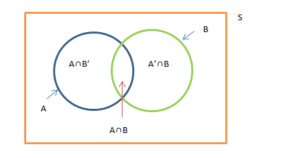
\includegraphics[width=\columnwidth] {independence.png}
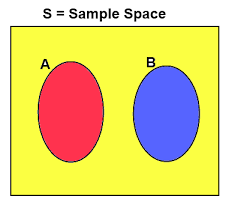
\includegraphics[width=\columnwidth] {ind.png}

\end{figure}


\subsection{ Gaussian Random numbers generation}
\\
\\
\\

let  sample size is 1000
Approach is first generated multivariate gaussian random variables and also data set is generated and then using the formula and generation concept is used for sum of 2 random variables as well.
Then graph is made for simulated as well as theoritical and it is colliding with 1000 random numbers generation
\\
\\
\\
\\
\begin{figure}

\includegraphics[width=\columnwidth] {data.png}
\includegraphics[width=\columnwidth] {sumof.png}
\includegraphics[width=\columnwidth] {simulated.png}
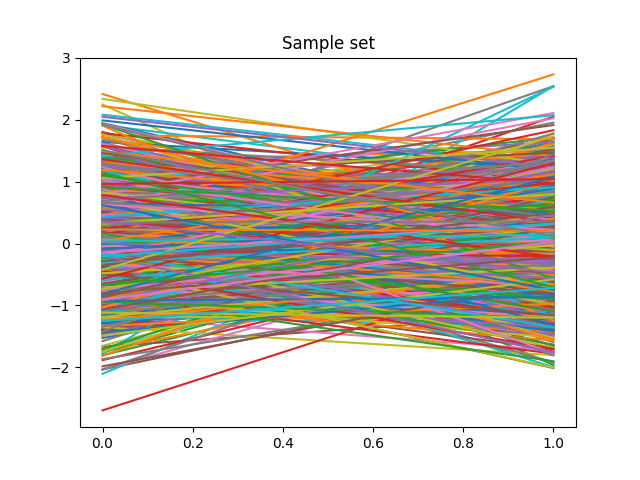
\includegraphics[width=\columnwidth] {sampleset.png}
\end{figure}

U is here sum of 2 gaussian random variables.
we can see that sum of 2 gaussian random variables is also gaussian
We can increase the number of samples in order to get more appropriate results.Here, graph colliding which is implying same i. e simulated and actual probability  More collision implies more appropriate results.
\end{document}

        

